\documentclass[11pt]{charter}

% El títulos de la memoria, se usa en la carátula y se puede usar el cualquier lugar del documento con el comando \ttitle
\titulo{Reproductor de audio digital con control de velocidad de reproducción} 

% Nombre del posgrado, se usa en la carátula y se puede usar el cualquier lugar del documento con el comando \degreename
\posgrado{Carrera de Especialización en Sistemas Embebidos} 
%\posgrado{Carrera de Especialización en Internet de las Cosas} 
%\posgrado{Carrera de Especialización en Intelegencia Artificial}
%\posgrado{Maestría en Sistemas Embebidos} 
%\posgrado{Maestría en Internet de las cosas}

% Tu nombre, se puede usar el cualquier lugar del documento con el comando \authorname
\autor{Florencia Battocchia} 

% El nombre del director y co-director, se puede usar el cualquier lugar del documento con el comando \supname y \cosupname y \pertesupname y \pertecosupname
\director{Pablo Slavkin}
\pertenenciaDirector{pertenencia} 
% FIXME:NO IMPLEMENTADO EL CODIRECTOR ni su pertenencia
\codirector{} % si queda vacio no se deberíá incluir 
\pertenenciaCoDirector{}

% Nombre del cliente, quien va a aprobar los resultados del proyecto, se puede usar con el comando \clientename y \empclientename
\cliente{Matias Battocchia}
\empresaCliente{Cliente particular}

% Nombre y pertenencia de los jurados, se pueden usar el cualquier lugar del documento con el comando \jurunoname, \jurdosname y \jurtresname y \perteunoname, \pertedosname y \pertetresname.
\juradoUno{Nombre y Apellido (1)}
\pertenenciaJurUno{pertenencia (1)} 
\juradoDos{Nombre y Apellido (2)}
\pertenenciaJurDos{pertenencia (2)}
\juradoTres{Nombre y Apellido (3)}
\pertenenciaJurTres{pertenencia (3)}
 
\fechaINICIO{22 de junio de 2020}		%Fecha de inicio de la cursada de GdP \fechaInicioName
\fechaFINALPlanificacion{22 de Agosto de 2020} 	%Fecha de final de cursada de GdP
\fechaFINALTrabajo{1 de junio de 2021}		%Fecha de defensa pública del trabajo final

\newcolumntype{L}[1]{>{\raggedright\let\newline\\\arraybackslash\hspace{0pt}}m{#1}}
\newcolumntype{C}[1]{>{\centering\let\newline\\\arraybackslash\hspace{0pt}}m{#1}}
\newcolumntype{R}[1]{>{\raggedleft\let\newline\\\arraybackslash\hspace{0pt}}m{#1}}

\begin{document}

\maketitle
\thispagestyle{empty}
\pagebreak


\thispagestyle{empty}
{\setlength{\parskip}{0pt}
\tableofcontents{}
}
\pagebreak


\section{Registros de cambios}
\label{sec:registro}


\begin{table}[ht]
\label{tab:registro}
\centering

\begin{tabularx}{\linewidth}{@{}|c|X|c|@{}}
\hline
\rowcolor[HTML]{C0C0C0} 
Revisión & \multicolumn{1}{c|}{\cellcolor[HTML]{C0C0C0}Detalles de los cambios realizados} & Fecha      \\ \hline
1.0      & Creación del documento                                                          & 22/06/2020 \\ \hline
1.1      & Se modifica el título del documento \newline                                                                                Se modifica el Acta de constitución del proyecto \newline                                                                               
Se modifica la Descripción técnica-conceptual del proyecto a realizar \newline                                                                               
Se realiza la tabla de Identificación y análisis de los interesados \newline                                                                               
Se modifican las secciones 1,2,3 y 5 & 31/07/2020 \\ \hline
1.2      & Se realiza el diagrama de Activity On Node \newline                                                                              
Se realiza el diagrama de Gantt\newline                                                                              
Se realiza la matriz de recursos materiales \newline                                                                              
Se realiza el presupuesto detallado del proyecto \newline                                                                              
Se realiza la matriz de responsables & 04/08/2020\\ \hline
1.3      & Se realiza la gestión de riesgos \newline                                                                              
Se realiza la gestión de calidad\newline                                                                              
Se realiza la comunicación del proyecto \newline                                                                              
Se realiza la gestión de compras \newline                                                                              
Se realiza el seguimiento y control \newline                                                                              
Se realiza el proceso de cierre & 08/08/2020\\ \hline

\end{tabularx}
\end{table}

\pagebreak



\section{Acta de constitución del proyecto}
\label{sec:acta}

\begin{flushright}
Buenos Aires, \fechaInicioName
\end{flushright}

\vspace{2cm}

Por medio de la presente se acuerda con la Ing. \authorname\hspace{1px} que su Trabajo Final de la \degreename\hspace{1px} se titulará ``\ttitle'', consistirá esencialmente en el prototipo preliminar de un dispositivo que almacena y reproduce un archivo de audio digital al cual se le podrá variar la velocidad de reproduccion del audio de forma permanente o temporal, y tendrá un presupuesto preliminar estimado de 600 hs de trabajo y \$243.550, con fecha de inicio \fechaInicioName\hspace{1px} y fecha de presentación pública \fechaFinalName.

Se adjunta a esta acta la planificación inicial.

\vfill

% Esta parte se construye sola con la información que hayan cargado en el preámbulo del documento y no debe modificarla
\begin{table}[ht]
\centering
\begin{tabular}{ccc}
\begin{tabular}[c]{@{}c@{}}Ariel Lutenberg \\ Director posgrado FIUBA\end{tabular} &  & \begin{tabular}[c]{@{}c@{}}\clientename \\ \empclientename \end{tabular} \vspace{2.5cm} \\ 
\multicolumn{3}{c}{\begin{tabular}[c]{@{}c@{}} \supname \\ Director del Trabajo Final\end{tabular}} \vspace{2.5cm} \\
\begin{tabular}[c]{@{}c@{}}\jurunoname \\ Jurado del Trabajo Final\end{tabular}     &  & \begin{tabular}[c]{@{}c@{}}\jurdosname\\ Jurado del Trabajo Final\end{tabular}  \vspace{2.5cm}  \\
\multicolumn{3}{c}{\begin{tabular}[c]{@{}c@{}} \jurtresname\\ Jurado del Trabajo Final\end{tabular}} \vspace{.5cm}                                                                     
\end{tabular}
\end{table}




\section{Descripción técnica-conceptual del proyecto a realizar}
\label{sec:descripcion}

\begin{consigna}{black}
Los primeros reproductores digitales para discjockeys aparecen a finales de los 80, su finalidad es poder reproducir la música almacenada en CDs de audio de manera similar a como se puede hacer con los platos giradiscos, es decir, pudiendo modificar la velocidad a la que se reproduce el tema para acompasarlo a otro ya sonando.

En 1993 comienza en este tipo de aparatos una fuerte revolución de la mano de Pioneer, que comercializa el CDJ-300, primer reproductor de la gama CDJ, gama que posteriormente ha dominado el mercado profesional de reproductores para DJ. Denon también desde el año 93 ha lanzado reproductores profesionales de gran aceptación, siendo la segunda marca en importancia por detrás de Pioneer en el mercado profesional.

En 2001 Pioneer volvió a revolucionar el mercado con el CDJ-1000, un reproductor de CDs capaz de emular más que cualquier otro producto lanzado hasta el momento el funcionamiento de un plato giradiscos gracias a que con su jog de gran tamaño se podían emular las técnicas de scratch que se realizan con platos y vinilos. 

A partir del año 2002 comienzan a surgir reproductores profesionales con capacidad para reproducir archivos MP3. Desde el año 2007 la capacidad de reproducir archivos MP3 comienza a convertirse en algo habitual en casi todos los reproductores, que ya son capaces de leer este tipo de archivos desde discos CD-R, pendrives USB o tarjetas de memoria. En la actualidad muchos dispositivos son capaces también de leer otros formatos como el M4A o el AAC, así como formatos sin compresión como WAV o AIFF.

En los últimos 5 años se han popularizado también los reproductores que pueden ser empleados como controladores MIDI con software para Djs.

Si bien en el mercado existe una gran variedad de estos equipos y con múltiples funciones(\textit{display, play/pause,CUE, track search, autocue,pitch control, pitch bend, master tempo, tempo range, jogwheel, loop, hot cue, navegación, efectos, slip}) son importados y extremadamente caros por ejemplo se muestra en la figura \ref{fig:Pioneer} un equipo Pioneer Cdj-2000 Nexus, que cuesta \$454.400

\begin{figure}[htpb]
\centering 
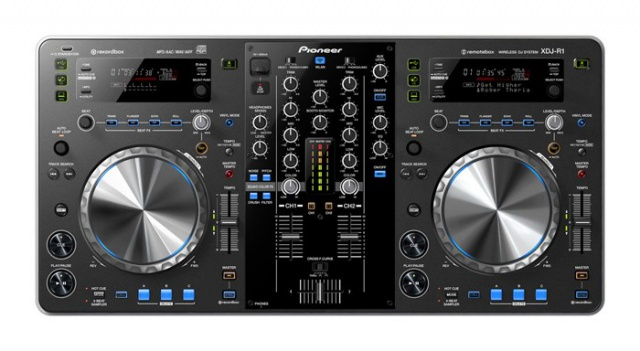
\includegraphics[width=.7\textwidth]{./Figuras/reproductordigital.jpeg}
\caption{Pioneer Cdj-2000 Nexus}
\label{fig:Pioneer}
\end{figure}

El presente proyecto se destaca especialmente por desarrollar una alternativa económica y que mantenga la funcionalidad simple del vinilo pero en forma digital, implementando las funcionalidades de \textit{play/pause, pitch control, pitch Bend}. El control \textit{play/pause} se realiza con un botón y su función es iniciar la reproducción o ponerla en pausa. El \textit{pitch control} se lleva a cabo con un potenciómetro deslizante y su función es la de modificar la velocidad de reproducción de la canción, posicionado en la parte central de su recorrido, la velocidad de reproducción no es afectada, deslizándolo hacia abajo aumenta y hacia arriba disminuye la velocidad de reproducción del audio. El control \textit{ pitch Bend} se realiza con dos botones marcados como +  y - , mientras se pulsan la velocidad de reproducción varía momentaneamente, uno la aumenta y el otro la disminuye.

Un diagrama general del trabajo se presenta en la figura \ref{fig:diagBloques}. El procesador de audio digital se encuentra representado por el bloque amarillo, mientras que en los bloques color azul se encuentra representado el ambiente con el cual interactúa el procesador. En la entrada del procesador se encuentra la consola que contiene la interfaz con el usuario y la unidad de almacenamiento que contiene el audio en formato wav PCM (\textit{Pulse-Code Modulation}). El procesador lee el audio almacenado y lo procesa según los eventos que recibe de la consola. En la salida se encuentra el DAC que convierte la señal de digital a analogica y se le aplica un filtro de reconstrucción. La salida de audio presenta formato RCA y se conecta a un equipo con entrada line-in que pre-amplifica la señal y permite escuchar la canción como por ejemplo un \textit{mixer} (mezcladora), este se encuentra en el recuadro verde y no pertene al desarrollo del proyecto. 

\begin{figure}[htpb]
\centering 
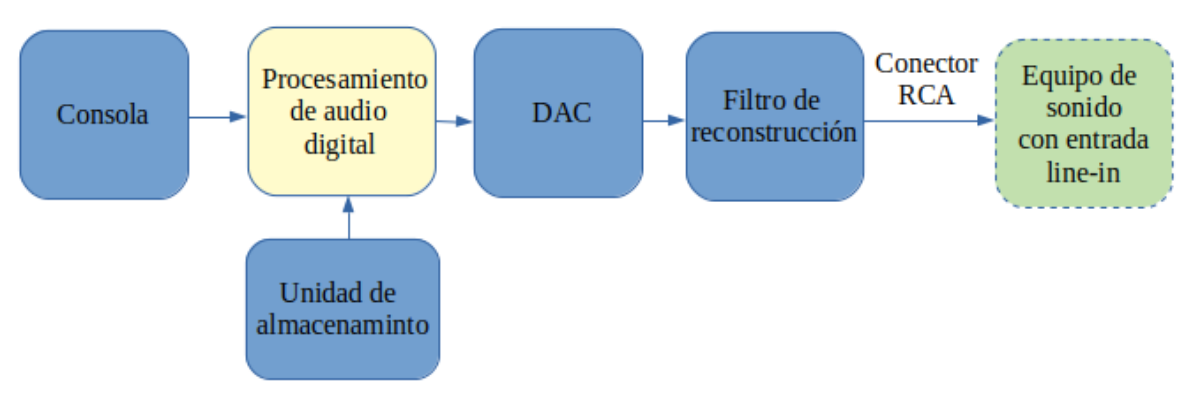
\includegraphics[width=.9\textwidth]{./Figuras/diagBloquesDSP.png}
\caption{Diagrama general del equipo.}
\label{fig:diagBloques}
\end{figure}

En la seguiente figura \ref{fig:consola} se detalla la interfaz con el usurio, donde el potenciometro lineal varía la velocidad de reproducción del audio de forma permanente (\textit{pitch control}), aumentando la velocidad cuando se de desplaza hacia abajo, produciendo un sonido mas agudo y disminuyendo la velocidad cuando se lo desplaza hacia arriba produciendo un sonido mas grave. Los botonos con símbolos menos (-) y mas (+) cambian la velocidad de reproducción del audio de forma temportal mientra se los mantiene pulsados (\textit{pitch bend}), también se puede observar en esta figura el botón de play/pausa.

\begin{figure}[H]
\centering 
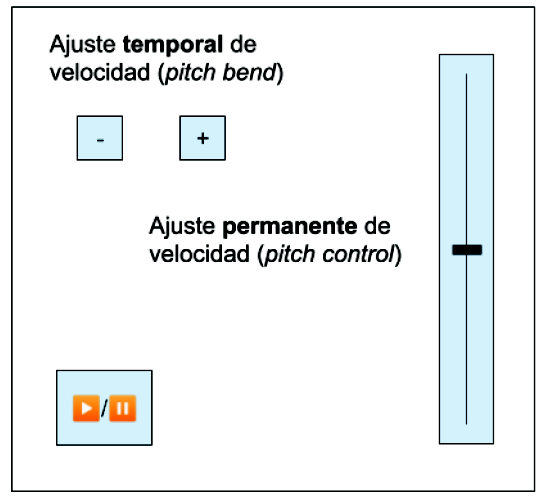
\includegraphics[width=.5\textwidth]{./Figuras/interfaz.png}
\caption{Interfaz de usuario.}
\label{fig:consola}
\end{figure}
 
\end{consigna}
\section{Identificación y análisis de los interesados}
\label{sec:interesados}

\begin{consigna}{black} 

\begin{table}[ht]
%\caption{Identificación de los interesados}
%\label{tab:interesados}
\begin{tabularx}{\linewidth}{@{}|l|X|X|l|@{}}
\hline
\rowcolor[HTML]{C0C0C0} 
Rol           & Nombre y Apellido & Organización 	& Puesto 	\\ \hline
Cliente       & \clientename      &\empclientename	&        	\\ \hline
Responsable   & \authorname       & FIUBA        	& Alumno 	\\ \hline
Orientador    & \supname	      & \pertesupname 	& Director	Trabajo final \\ \hline
Usuario final & \clientename      & \empclientename	&        	\\ \hline
\end{tabularx}
\end{table}


\end{consigna}



\section{1. Propósito del proyecto}
\label{sec:proposito}

\begin{consigna}{black}
El propósito de este proyecto es desarrollar un reproductor de audio digital con control de velocidad de reproducción para obtener un dispositivo de características similares a las del vinilo en forma digital a un costo inferior a los existentes en el mercado. 
\end{consigna}

\section{2. Alcance del proyecto}
\label{sec:alcance}

\begin{consigna}{black}
El siguiente proyecto incluye:
\begin{itemize}
\item Soporte para almacenamiento de audio.
\item Control de velocidad de la reproducción del audio de forma temporal.
\item Control de velocidad de la reproducción del audio de forma permanente.
\item Reproducción y pausa del audio.
\item Salida de audio por dos canales.
\end{itemize}

El presente proyecto no incluye:
\begin{itemize}
\item Formatos de audio comprimido MP3, AAC, FLAC, ALAC.
\item Pantalla LCD con información de la pista, tiempo transcurrido, tiempo restante, valor de ajuste de velocidad, forma de onda.
\item Controles adicionales para seleccionar y cargar pistas.
\end{itemize}
\end{consigna}

\section{3. Supuestos del proyecto}
\label{sec:supuestos}

\begin{consigna}{black}
Para el desarrollo del presente proyecto se supone que:

\begin{itemize}
\item Se tiene acceso al instrumental de testeo necesario (osciloscopio, analizador de espectro)
\item Se podrán dedicar entre 2hs y 4hs diarias al desarrollo del proyecto fuera del horario laboral
\end{itemize}
\end{consigna}

\section{4. Requerimientos}
\label{sec:requerimientos}
\begin{consigna}{black}
\begin{enumerate}
\item Requerimientos del sistema operativo:
	\begin{enumerate}
	\item Se deberá utilizar un sistema operativo de tiempo real.
	\end{enumerate}
\item Requerimientos de Hardware:
	\begin{enumerate}
	\item Se deberá utilizará la CIAA-NXP como computadora principal.
	\item Se deberá utilizar un DAC de audio que genere la señal \textit{Master Clock} de la interfaz I2S internamente 
	\item Deberá utilizar un conector RCA estéreo para conectar el dispositivo a un equipo con entrada  line-in.
	\end{enumerate}
\item Requerimientos de la interfaz de usuario:
	\begin{enumerate}
	\item Deberá tener un botón de reproducción/pausa del audio.
	\item Deberá tener 2 botones de ajuste temporal de velocidad que disminuyen o incrementan la velocidad mientras se encuentran pulsados.
	\item Deberá tener un potenciómetro lineal para el ajuste permanente de velocidad.	
	\end{enumerate}
\item Requerimientos de fuente de audio:
	\begin{enumerate}
	\item Se deberá almacenar el archivo de audio en en una memoria SD
	\item El archivo de audio deberá tener formato .wav con 44100 Hz, calidad estéreo de 16 bits.
	\item El archivo de audio deberá tener formato PCM.
	\end{enumerate}
\item Requerimientos de salida de sonido:
	\begin{enumerate}
	\item La velocidad normal de reproducción del audio deberó ser de 44100 Hz.
	\item El \textit{pith control} deberá aumentar o disminuir la velocidad normal de reproducción hasta un un 8\%.
	\item El \textit{pinch bend} deberá aumentar o disminuir la velocidad normal de reproducción un 5\%.
	\item Se deberá implementar dos canales de salida.
	\item Se deberá presentar un nivel de distorsión mayor a 40 DB.
	\item El nivel de salida deberá ser de 2,0 Vrms.
	\end{enumerate}
\item Requerimientos de alimentacion:
	\begin{enumerate}
	\item La alimentación deberá ser de 5 VCC por medio de USB.
	\end{enumerate}
\end{enumerate}
\end{consigna}

\section{5. Entregables principales del proyecto}
\label{sec:entregables}

\begin{consigna}{black}
\begin{itemize}
\item Manual de uso
\item Código fuente
\item Esquemático de conexionado.
\item Informe final

\end{itemize}

\end{consigna}

\section{6. Desglose del trabajo en tareas}
\label{sec:wbs}

\begin{consigna}{black}

\begin{enumerate}
\item Planificación del proyecto (20hs)
	\begin{enumerate}
	\item Realizar la planificación del proyecto (20hs)
	\end{enumerate}
\item Recopilación general de información sobre el proyecto (80 hs)
	\begin{enumerate}
	\item Realizar el análisis y elección de la electrónica y el microcontrolador a utilizar (10hs)
	\item Investigar sobre algoritmos de procesamiento de señales digitales en tiempo real (30hs)
	\item Investigar sobre técnicas de conversión de señal digital a analógica : DAC, PWM o r2r network 		dac (30hs)
	\item Buscar información sobre procesadores de audio comerciales (10 hs)
	\end{enumerate}
\item Diseño de hardware (20 hs)
	\begin{enumerate}
	\item Diseño esquemático de conexionado. (20hs)
	\end{enumerate}
\item Implementación de la consola (50hs)
	\begin{enumerate}
	\item Realizar el circuito electrónico de la interfaz de usuario (15hs)
	\item Testeo de del circuito electrónico. (5hs)
	\item Realizar la lectura de las entradas de la interfaz de usuario. (30hs)
	\end{enumerate}
\item Adquisiscion de audio de la memoria SD (32hs)
	\begin{enumerate}
	\item Realizar circuito electrónico para conectar la memoria SD. (5hs)
	\item Testeo del circuito electrónico. (5hs)
	\item Burcar audio que cumpla con el requisito 4. y almacenarlo en la memoria SD. (2hs)
	\item Realizar la lectura del audio almacenado en la tarjeta SD. (20hs)
	\end{enumerate}
\item Implementació del sistema operativo (40hs)
	\begin{enumerate}
	\item Implementar sistema operativo RTEMS (20hs)
	\item Implementar manejo de las interrupciones provenientes de la interfaz de usuario (20hs) 
	\end{enumerate}
\item Implementación de algoritmos de procesamiento de señales (100hs)
	\begin{enumerate}
	\item Implementar algoritmo de re-muestreo para controlar la velocidad de reproducción del audio. (40hs)
	\item Implementar algoritmo de filtro de interpolación.(40hs)
	\item Testeo de los algoritmos desarrollados (20 hs)
	\end{enumerate}
\item Salida de audio (68 hs)
	\begin{enumerate}
	\item Desarrollo librería de generación del DAC por I2S (40hs)
	\item Realizar circuito electrónico del DAC externo en protoboard. (5hs)
	\item Testeo de la salida del DAC con osciloscopio y analizador de espectros. (5 hs)
	\item Realizar circuito electrónico del filtro de reconstrucción en protoboard. (5hs)
	\item Realizar circuito electrónico del conector RCA en protoboard. (5hs)
	\item Testeo de los circuitos electrónico. (8hs)
	\end{enumerate}
\item Integración del sistema (30hs)
	\begin{enumerate}
	\item Integración de los módulos del sistema (20hs).
	\item Testeo de funcionamiento (10hs).
	\end{enumerate}
\item Pruebas (80hs)
	\begin{enumerate}
	\item Desarrollar herramientas de testeo, debug y validación. (40 hs)
	\item Realizar las pruebas de validación del sistema (40 hs)
	\end{enumerate}
\item Documentación (80 hs)
	\begin{enumerate}
	\item Realizar el informe final del proyecto (50hs)
	\item Realizar el manual de uso (30hs)
	\end{enumerate}
\end{enumerate}

Cantidad total de horas: (600 hs)

\end{consigna}

\section{7. Diagrama de Activity On Node}
\label{sec:AoN}

\begin{consigna}{black}
En la siguiente figura \ref{fig:AoN} observa el diagrama de Activity On Node.

\begin{figure}[htpb]
\centering 
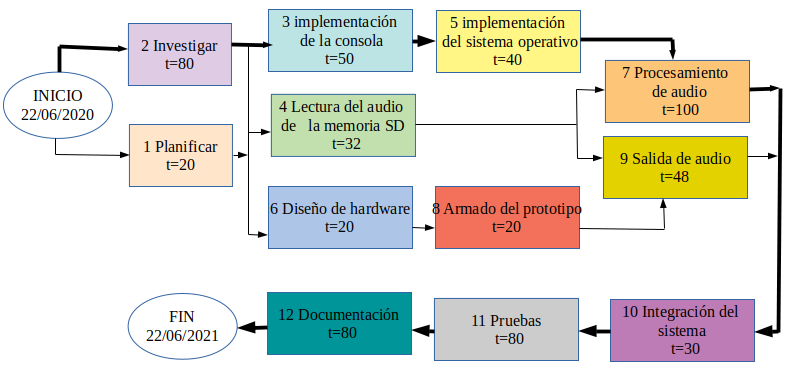
\includegraphics[width=.9\textwidth]{./Figuras/AoN.png}
\caption{Diagrama en \textit{Activity on Node}}
\label{fig:AoN}
\end{figure}


Los tiempos expresados en el diagrama se encuentran en horas. El color de cada recuadro
representa el grupo de tareas contenidas en el punto.

\end{consigna}



\section{8. Diagrama de Gantt}
\label{sec:gantt}
\begin{consigna}{black}

A continuación se observa el diagrama de Gantt \ref{fig:gant1}

\begin{figure}[H]
\centering 
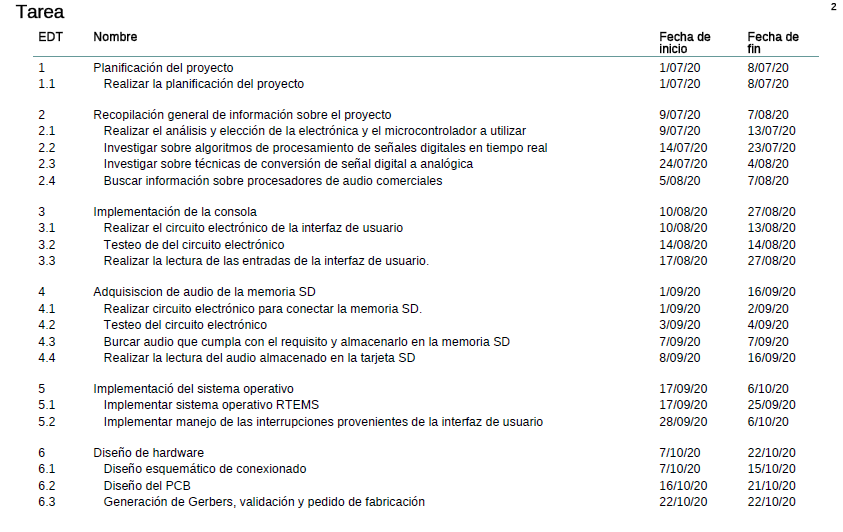
\includegraphics[width=1.1\textwidth]{./Figuras/gant1.png}
\caption{Diagrama de \textit{Gantt}}
\label{fig:gant1}
\end{figure}

\begin{figure}[H]
\centering 
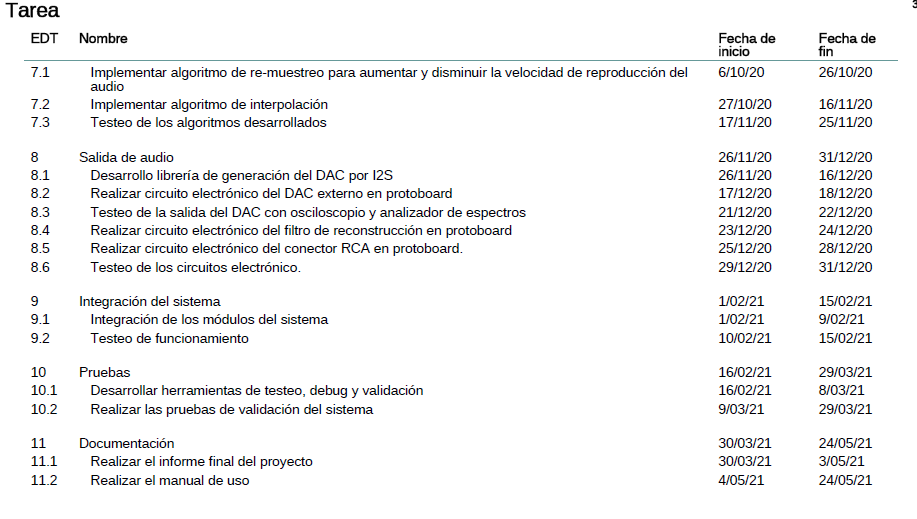
\includegraphics[width=1.1\textwidth]{./Figuras/gant2.png}
\caption{Diagrama de \textit{Gantt continuación}}
\label{fig:gant1}
\end{figure}

\begin{figure}[H]
\centering 
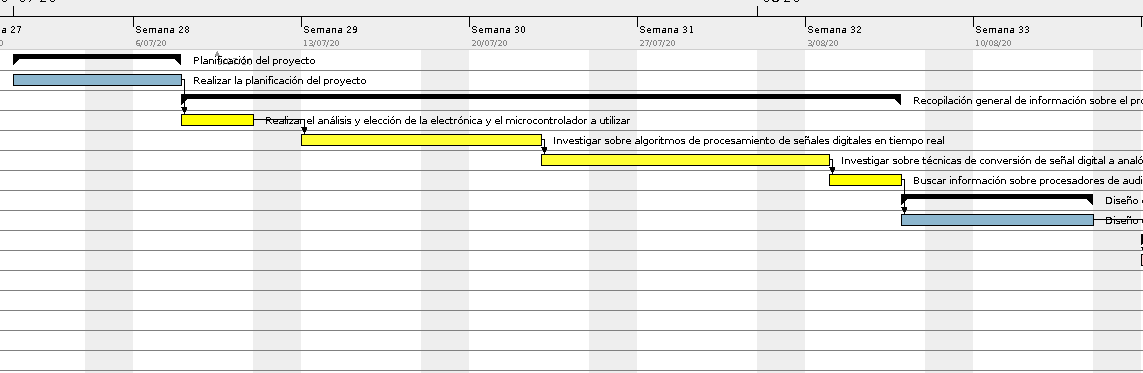
\includegraphics[width=1.5\textwidth,angle=270]{./Figuras/gant3.png}
\caption{Diagrama de \textit{Gantt continuación}}
\label{fig:gant1}
\end{figure}

\begin{figure}[H]
\centering 
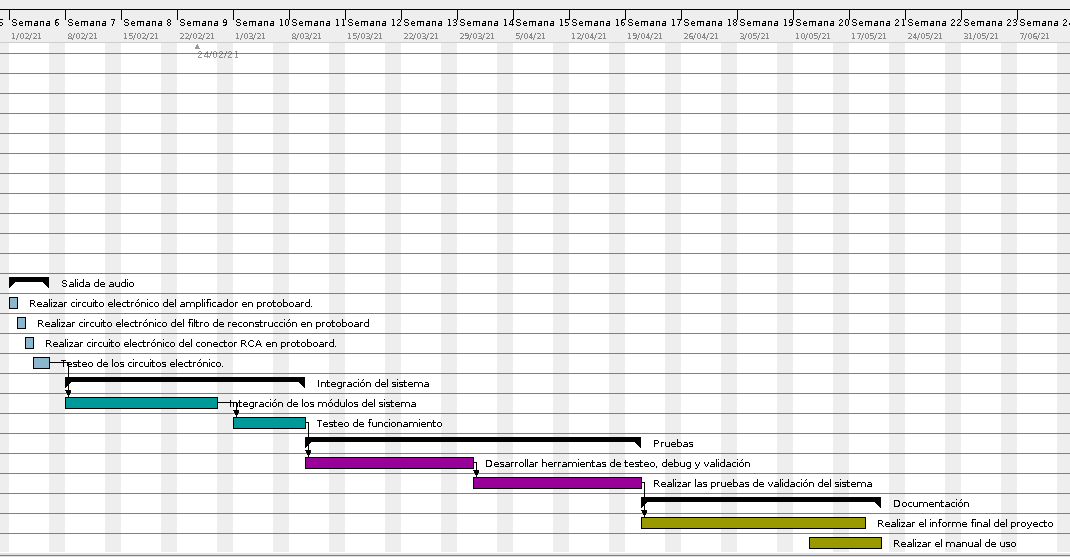
\includegraphics[width=1.5\textwidth,angle=-90]{./Figuras/gant4.png}
\caption{Diagrama de \textit{Gantt continuación}}
\label{fig:gant1}
\end{figure}

\begin{figure}[H]
\centering 
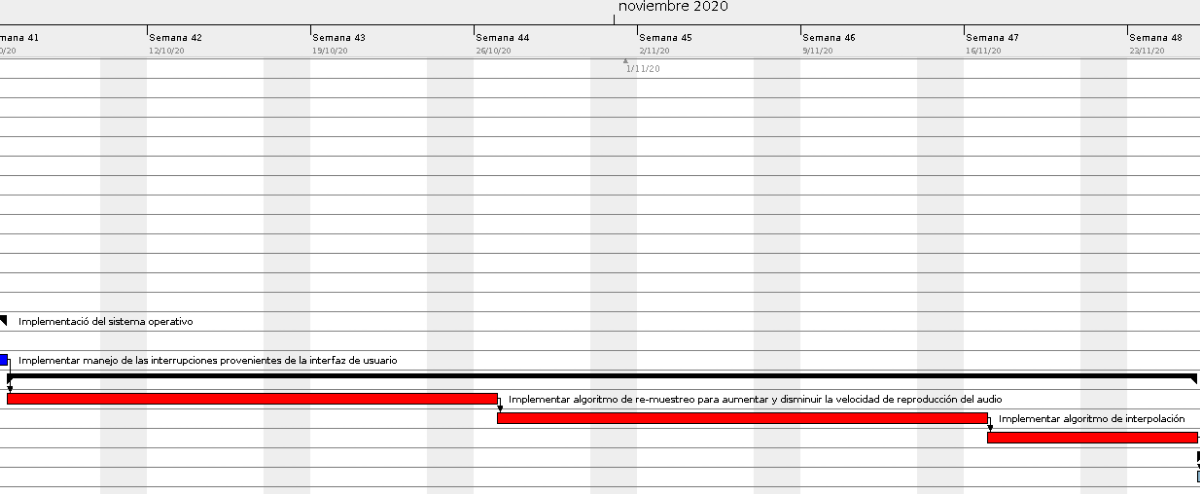
\includegraphics[width=1.5\textwidth,angle=-90]{./Figuras/gant5.png}
\caption{Diagrama de \textit{Gantt continuación}}
\label{fig:gant1}
\end{figure}
\begin{figure}[H]
\centering 
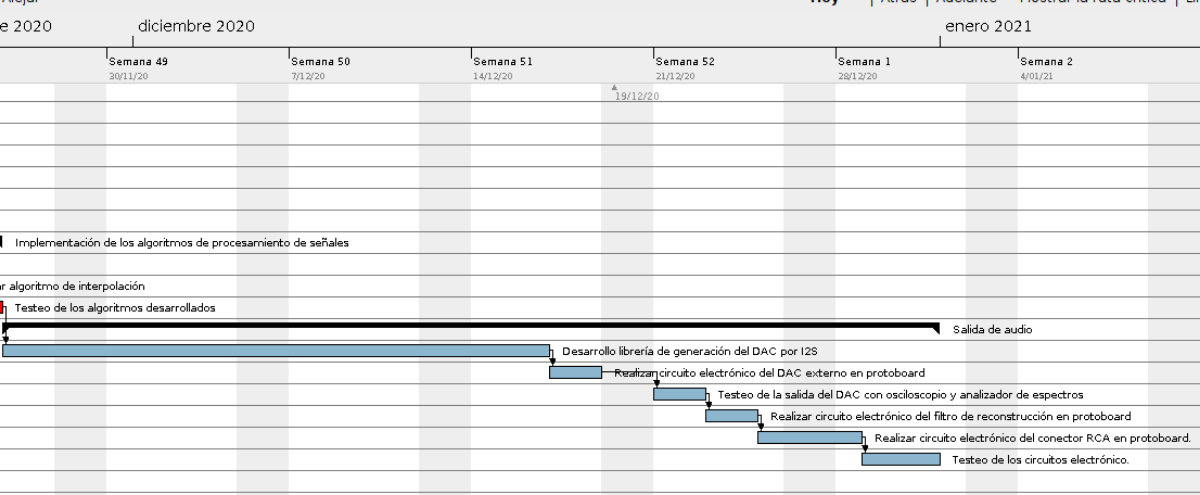
\includegraphics[width=1.5\textwidth,angle=-90]{./Figuras/gant6.png}
\caption{Diagrama de \textit{Gantt continuación}}
\label{fig:gant1}
\end{figure}
\begin{figure}[H]
\centering 
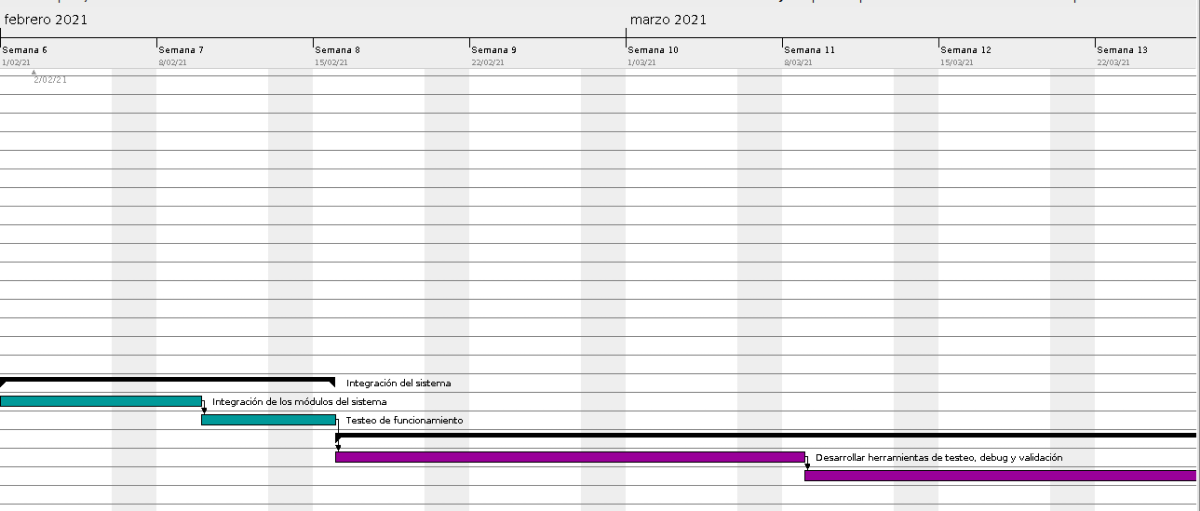
\includegraphics[width=1.5\textwidth,angle=-90]{./Figuras/gant7.png}
\caption{Diagrama de \textit{Gantt continuación}}
\label{fig:gant1}
\end{figure}
\begin{figure}[H]
\centering 
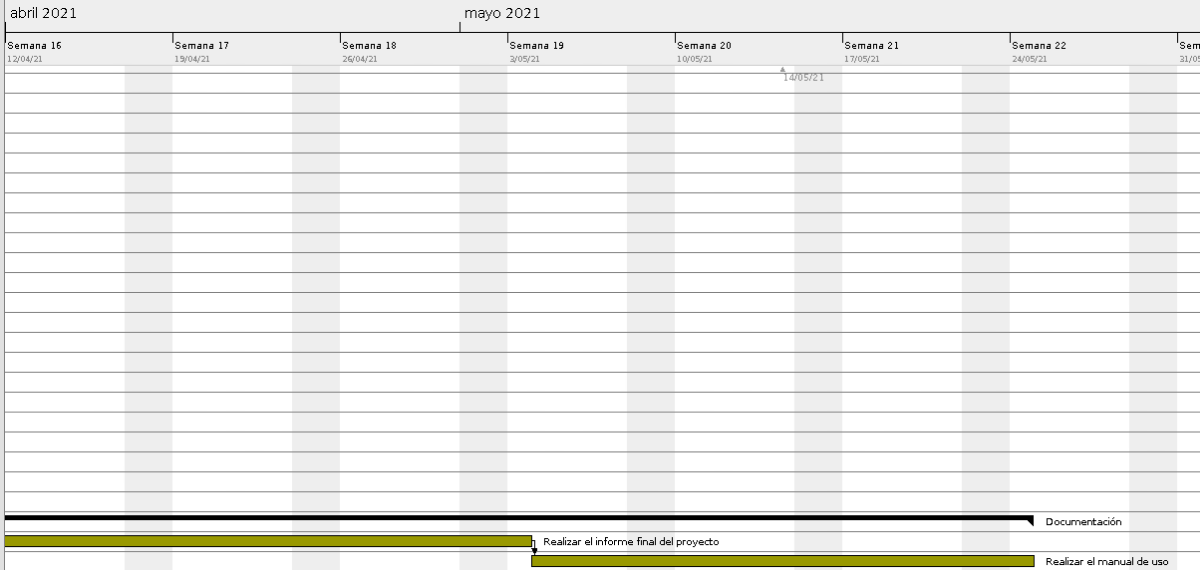
\includegraphics[width=1.5\textwidth,angle=-90]{./Figuras/gant8.png}
\caption{Diagrama de \textit{Gantt continuación}}
\label{fig:gant1}
\end{figure}
\end{consigna}

\section{9. Matriz de uso de recursos de materiales}
\label{sec:recursos}
\begin{consigna}{black}


\begin{longtable}{|c|C{4cm}|c|c|c|c|}

% aquí añadimos el encabezado de la primera hoja.
\hline
\rowcolor[HTML]{C0C0C0} 
\cellcolor[HTML]{C0C0C0}                                                                       & \cellcolor[HTML]{C0C0C0}                                                           & \multicolumn{4}{c|}{\cellcolor[HTML]{C0C0C0}Recursos Requeridos (Horas)}                               \\ \cline{3-6} 
\rowcolor[HTML]{C0C0C0} 
\multirow{-2}{*}{\cellcolor[HTML]{C0C0C0}\begin{tabular}[c]{@{}c@{}}Código\\ WBS\end{tabular}} & \multirow{-2}{*}{\cellcolor[HTML]{C0C0C0}Nombre de la tarea}                       & PC & EDU-CIAA-NXP & Osciloscopio & \begin{tabular}[c]{@{}c@{}}Analizador\\ de\\ espectros\end{tabular}\\
\hline \hline
\endfirsthead

% aquí añadimos el encabezado del resto de hojas.
\hline
\rowcolor[HTML]{C0C0C0} 
\cellcolor[HTML]{C0C0C0}                                                                       & \cellcolor[HTML]{C0C0C0}                                                           & \multicolumn{4}{c|}{\cellcolor[HTML]{C0C0C0}Recursos Requeridos (Horas)}                               \\ \cline{3-6} 
\rowcolor[HTML]{C0C0C0} 
\multirow{-2}{*}{\cellcolor[HTML]{C0C0C0}\begin{tabular}[c]{@{}c@{}}Código\\ WBS\end{tabular}} & \multirow{-2}{*}{\cellcolor[HTML]{C0C0C0}Nombre de la tarea}                       & PC & EDU-CIAA-NXP & Osciloscopio & \begin{tabular}[c]{@{}c@{}}Analizador\\ de\\ espectros\end{tabular} \\
\hline \hline
\endhead

% aquí añadimos el fondo de todas las hojas, excepto de la última.
\multicolumn{2}{c}{Sigue en la página siguiente.}
\endfoot

% aquí añadimos el fondo de la última hoja.
\endlastfoot

% aquí añadimos el cuerpo de la tabla.
\rowcolor[HTML]{CBCEFB} 
1                                                                                              & Planificación del proyecto                                                         &    &              &              &                                                                     \\ \hline
1.1                                                                                            & Realizar la planificación del proyecto                                             & 20 &              &              &                                                                     \\ \hline
\rowcolor[HTML]{CBCEFB} 
2                                                                                              & Recopilación general de información sobre el proyecto                              &    &              &              &                                                                     \\ \hline
2.1                                                                                            & Realizar el análisis y elección de la electrónica y el microcontrolador a utilizar & 10 &              &              &                                                                     \\ \hline
2.2                                                                                            & Investigar sobre algoritmos de procesamiento de señales digitales en tiempo real   & 30 &              &              &                                                                     \\ \hline
2.3                                                                                            & Investigar sobre técnicas de conversión de señal digital a analógica               & 30 &              &              &                                                                     \\ \hline
2.4  & Buscar información sobre procesadores de audio comerciales  & 10 &   & &                                                                    \\ \hline

\rowcolor[HTML]{CBCEFB} 
3                                                                                              & Diseño de hardware                                                                 &    &              &              &                                                                     \\ \hline
3.1                                                                                            & Diseño esquemático de conexionado.                                                 & 20 &              &              &                                                                     \\ \hline
\rowcolor[HTML]{CBCEFB} 
4                                                                                              & Implementació de la consola                                                        &    &              &              &                                                                     \\ \hline
4.1                                                                                            & Realizar el circuito electrónico de la interfaz de usuario                         &    &              &              &                                                                     \\ \hline
4.2                                                                                            & Testeo de del circuito electrónico                                                 &    &              &              &                                                                     \\ \hline
4.3                                                                                            & Realizar la lectura de las entradas de la interfaz de usuario                      & 30 & 30           &              &                                                                     \\ \hline
\rowcolor[HTML]{CBCEFB} 
5                                                                                              & Adquisiscion de audio de la memoria SD                                             &    &              &              &                                                                     \\ \hline
5.1                                                                                            & Realizar circuito electrónico para conectar la memoria SD. (5hs)                   &    &              &              &                                                                     \\ \hline
5.2                                                                                            & Testeo del circuito electrónico.                                                   &    &              &              &                                                                     \\ \hline
5.3                                                                                            & Burcar audio que cumpla con el requerimiento  y almacenarlo en la memoria SD.      & 2  &              &              &                                                                     \\ \hline
5.4                                                                                            & Realizar la lectura del audio almacenado en la tarjeta SD.                         & 20 & 20           &              &                                                                     \\ \hline
\rowcolor[HTML]{CBCEFB} 
6                                                                                              & Implementació del sistema operativo                                                &    &              &              &                                                                     \\ \hline
6.1                                                                                            & Implementar sistema operativo RTEMS                                                & 20 & 20           &              &                                                                     \\ \hline
6.2                                                                                            & Implementar manejo de las interrupciones  provenientes de la interfaz de usuario   & 20 & 20           &              &                                                                     \\ \hline
\rowcolor[HTML]{CBCEFB} 
7                                                                                              & Implementación de los algoritmos de procesamiento de señales                       &    &              &              &                                                                     \\ \hline
7.1                                                                                            & Implementar algoritmo de re-muestreo para controlar la velocidad de reproducción   & 40 & 40           &              &                                                                     \\ \hline
7.2                                                                                            & Implementar algoritmo de interpolación.                                            & 40 & 40           &              &                                                                     \\ \hline
7.3  & Testeo de los algoritmos desarrollados         & 20 & 20    &              &                                                                     \\ \hline
\rowcolor[HTML]{CBCEFB} 
8                                                                                              & Salida de audio                                                                    &    &              &              &                                                                     \\ \hline
8.1  & Desarrollo de librería de generacion del DAC por I2S    & 40    & 40             &              &                                                                     \\ \hline
8.2  & Realizar circuito electrónico del DAC en protoboard    &     &              &              &                                                                     \\ \hline
8.3  & Testeo de la salida del DAC con osciloscopio y analizadior de espectro    &   &  & 3    &                                                                    2 \\ \hline
8.4                                                                                            & Realizar circuito electrónico del filtro de reconstrucción en protoboard           &    &              &              &                                                                     \\ \hline
8.5                                                                                            & Realizar circuito electrónico del conector RCA en protoboard                       &    &              &              &                                                                     \\ \hline
8.6                                                                                            & Testeo de los circuitos electrónico                                                &    &              & 4            &                                                                     \\ \hline
\rowcolor[HTML]{CBCEFB} 
9                                                                                              & Integración del sistema                                                            &    &              &              &                                                                     \\ \hline
9.1                                                                                            & Integración de los módulos del sistema                                             & 20 & 20           &              &                                                                     \\ \hline
9.2                                                                                            & Testeo de funcionamiento                                                           &    &              & 5            & 5                                                                   \\ \hline
\rowcolor[HTML]{CBCEFB} 
10                                                                                             & Pruebas                                                                            &    &              &              &                                                                     \\ \hline
10.1                                                                                           & Desarrollar herramientas de testeo, debug y validación.                            & 40 &              &              &                                                                     \\ \hline
10.2                                                                                           & Realizar las pruebas de validación del sistema                                     & 40 & 40           &              &                                                                     \\ \hline
\rowcolor[HTML]{CBCEFB} 
11                                                                                             & Documentación                                                                      &    &              &              &                                                                     \\ \hline
11.1                                                                                           & Realizar el informe final del proyecto                                             & 50 &              &              &                                                                     \\ \hline
11.2                                                                                           & Realizar el manual de uso                                                          & 30 &              &              &  


\\ % esta línea es importante para que deje un espacio entre la tabla y el nombre de la tabla.
\caption{Matriz de uso de recursos materiales.}

\label{ta:recursos}
\end{longtable}
\end{consigna}
\section{10. Presupuesto detallado del proyecto}
\label{sec:presupuesto}
\begin{table}[H]
\begin{tabular}{|l|c|c|c|}
\hline
\rowcolor[HTML]{C0C0C0} 
\multicolumn{4}{|c|}{\cellcolor[HTML]{C0C0C0}COSTOS DIRECTOS}                                                                \\ \hline
\rowcolor[HTML]{C0C0C0} 
\multicolumn{1}{|c|}{\cellcolor[HTML]{C0C0C0}Descripción} & Cantidad              & Valor unitario (\$)   & Valor total (\$) \\ \hline
EDU-CIAA-NXP                                              & 1                     & 4600                  & 4600             \\ \hline
memoria SD                                                & 1                     & 550                   & 550              \\ \hline
potenciómetro lineal                                      & 1                     & 220                   & 200              \\ \hline
DAC PCM5100A                                            & 1                     & 1000                   & 1000              \\ \hline
cable RCA                                                 & 1                     & 1000                  & 1000             \\ \hline
componentes varios                                        & \multicolumn{1}{l|}{} & 1000                  & 1000             \\ \hline
Hs/hombre                                                 & 600Hs                 & 300                   & 180000           \\ \hline
\multicolumn{3}{|c|}{SUBTOTAL}                                                                            & 187.350           \\ \hline
\rowcolor[HTML]{C0C0C0} 
\multicolumn{4}{|c|}{\cellcolor[HTML]{C0C0C0}COSTOS INDIRECTOS}                                                              \\ \hline
\rowcolor[HTML]{C0C0C0} 
\multicolumn{1}{|c|}{\cellcolor[HTML]{C0C0C0}Descripción} & Cantidad              & Valor unitario        & Valor total      \\ \hline
30\% de los costos directos                               & \multicolumn{1}{l|}{} & \multicolumn{1}{l|}{} & 56.205            \\ \hline
\multicolumn{3}{|c|}{SUBTOTAL}                                                                            &                  \\ \hline
\rowcolor[HTML]{C0C0C0} 
\multicolumn{3}{|c|}{\cellcolor[HTML]{C0C0C0}TOTAL}                                                       & 243.555           \\ \hline
\end{tabular}
\end{table}


\section{11. Matriz de asignación de responsabilidades}
\label{sec:responsabilidades}

\begin{longtable}{|c|C{4cm}|c|c|c|}
\hline
\rowcolor[HTML]{C0C0C0} 
\cellcolor[HTML]{C0C0C0}                                                                       & \cellcolor[HTML]{C0C0C0}                                                           & \multicolumn{3}{c|}{\cellcolor[HTML]{C0C0C0}Nombres y roles definidos en el proyecto}                                                                                                                                   \\ \cline{3-5} 
\rowcolor[HTML]{C0C0C0} 
\multirow{-2}{*}{\cellcolor[HTML]{C0C0C0}\begin{tabular}[c]{@{}c@{}}Código\\ WBS\end{tabular}} & \multirow{-2}{*}{\cellcolor[HTML]{C0C0C0}Nombre de la tarea}                       & \begin{tabular}[c]{@{}c@{}}Responsable\\  Florencia Battocchia\end{tabular} & \begin{tabular}[c]{@{}c@{}}Orientador\\ Pablo Slavkin\end{tabular} & \begin{tabular}[c]{@{}c@{}}Cliente\\  Matias Battocchia\end{tabular} \\ \hline
\endfirsthead
\hline
\rowcolor[HTML]{C0C0C0} 
\cellcolor[HTML]{C0C0C0}                                                                       & \cellcolor[HTML]{C0C0C0}                                                           & \multicolumn{3}{c|}{\cellcolor[HTML]{C0C0C0}Nombres y roles definidos en el proyecto}                                                                                                                                   \\ \cline{3-5} 
\rowcolor[HTML]{C0C0C0} 
\multirow{-2}{*}{\cellcolor[HTML]{C0C0C0}\begin{tabular}[c]{@{}c@{}}Código\\ WBS\end{tabular}} & \multirow{-2}{*}{\cellcolor[HTML]{C0C0C0}Nombre de la tarea}                       & \begin{tabular}[c]{@{}c@{}}Responsable\\  Florencia Battocchia\end{tabular} & \begin{tabular}[c]{@{}c@{}}Orientador\\ Pablo Slavkin\end{tabular} & \begin{tabular}[c]{@{}c@{}}Cliente\\  Matias Battocchia\end{tabular} \\ \hline
\endhead
\multicolumn{2}{c}{Sigue en la página siguiente.}
\endfoot
\endlastfoot
\rowcolor[HTML]{CBCEFB} 
1                                                                                              & Planificación del proyecto                                                         &                                                                             &                                                                    &                                                                      \\ \hline
1.1                                                                                            & Realizar la planificación del proyecto                                             & P                                                                           & A                                                                  & A                                                                    \\ \hline
\rowcolor[HTML]{CBCEFB} 
2                                                                                              & Recopilación general de información sobre el proyecto                              &                                                                             &                                                                    &                                                                      \\ \hline
2.1                                                                                            & Realizar el análisis y elección de la electrónica y el microcontrolador a utilizar & P                                                                           & I                                                                  & C                                                                    \\ \hline
2.2                                                                                            & Investigar sobre algoritmos de procesamiento de señales digitales en tiempo real   & P                                                                           & I                                                                  & I                                                                    \\ \hline
2.3                                                                                            & Investigar sobre técnicas de conversión de señal digital a analógica               & P                                                                           & I                                                                  & I                                                                    \\ \hline
2.4                                                                                            & Buscar información sobre procesadores de audio comerciales                         & P                                                                           & I                                                                  & I                                                                    \\ \hline
\rowcolor[HTML]{CBCEFB} 
3                                                                                              & Diseño de hardware                                                                 &                                                                             &                                                                    &                                                                      \\ \hline
3.1                                                                                            & Diseño esquemático de conexionado.                                                 & P                                                                           & A                                                                  & I                                                                    \\ \hline
\rowcolor[HTML]{CBCEFB} 
4                                                                                              & Implementació de la consola                                                        &                                                                             &                                                                    &                                                                      \\ \hline
4.1                                                                                            & Realizar el circuito electrónico de la interfaz de usuario                         & P                                                                           & I                                                                  & I                                                                    \\ \hline
4.2                                                                                            & Testeo de del circuito electrónico                                                 & P                                                                           & I                                                                  & I                                                                    \\ \hline
4.3                                                                                            & Realizar la lectura de las entradas de la interfaz de usuario                      & P                                                                           & I                                                                  & I                                                                    \\ \hline
\rowcolor[HTML]{CBCEFB} 
5                                                                                              & Adquisiscion de audio de la memoria SD                                             &                                                                             &                                                                    &                                                                      \\ \hline
5.1                                                                                            & Realizar circuito electrónico para conectar la memoria SD. (5hs)                   & P                                                                           & I                                                                  & I                                                                    \\ \hline
5.2                                                                                            & Testeo del circuito electrónico.                                                   & P                                                                           & I                                                                  & I                                                                    \\ \hline
5.3                                                                                            & Burcar audio que cumpla con el requerimiento  y almacenarlo en la memoria SD.      & P                                                                           & I                                                                  & C                                                                    \\ \hline
5.4                                                                                            & Realizar la lectura del audio almacenado en la tarjeta SD.                         & P                                                                           & I                                                                  & I                                                                    \\ \hline
\rowcolor[HTML]{CBCEFB} 
6                                                                                              & Implementació del sistema operativo                                                &                                                                             &                                                                    &                                                                      \\ \hline
6.1                                                                                            & Implementar sistema operativo RTEMS                                                & P                                                                           & I                                                                  & I                                                                    \\ \hline
6.2                                                                                            & Implementar manejo de las interrupciones  provenientes de la interfaz de usuario   & P                                                                           & I                                                                  & I                                                                    \\ \hline
\rowcolor[HTML]{CBCEFB} 
7                                                                                              & Implementación de los algoritmos de procesamiento de señales                       &                                                                             &                                                                    &                                                                      \\ \hline
7.1                                                                                            & Implementar algoritmo de re-muestreo para controlar la velocidad de reproducción   & P                                                                           & C                                                                  & I                                                                    \\ \hline
7.2                                                                                            & Implementar algoritmo de interpolación.                                            & P                                                                           & C                                                                  & I                                                                    \\ \hline
7.3                                                                                            & Testeo de los algoritmos desarrollados                                             & P                                                                           & I                                                                  & I                                                                    \\ \hline
\rowcolor[HTML]{CBCEFB} 
8                                                                                              & Salida de audio                                                                    &                                                                             &                                                                    &                                                                      \\ \hline
8.1                                                                                            & Desarrollo librería de generación del DAC por I2S                                  & P                                                                           & I                                                                  & I                                                                    \\ \hline
8.2                                                                                            & Realizar circuito electrónico del DAC externo en protoboard                        & P                                                                           & I                                                                  & I                                                                    \\ \hline
8.3                                                                                            & Testeo de la salida del DAC con osciloscopio y analizador de espectros             & P                                                                           & A                                                                  & I                                                                    \\ \hline
8.4                                                                                            & Realizar circuito electrónico del filtro de reconstrucción en protoboard           & P                                                                           & I                                                                  & I                                                                    \\ \hline
8.5                                                                                            & Realizar circuito electrónico del conector RCA en protoboard                       & P                                                                           & I                                                                  & I                                                                    \\ \hline
8.6                                                                                            & Testeo de los circuitos electrónico                                                & P                                                                           & I                                                                  & I                                                                    \\ \hline
\rowcolor[HTML]{CBCEFB} 
9                                                                                              & Integración del sistema                                                            &                                                                             &                                                                    &                                                                      \\ \hline
9.1                                                                                            & Integración de los módulos del sistema                                             & P                                                                           & I                                                                  & I                                                                    \\ \hline
9.2                                                                                            & Testeo de funcionamiento                                                           & P                                                                           & A                                                                  & I                                                                    \\ \hline
\rowcolor[HTML]{CBCEFB} 
10                                                                                             & Pruebas                                                                            &                                                                             &                                                                    &                                                                      \\ \hline
10.1                                                                                           & Desarrollar herramientas de testeo, debug y validación.                            & P                                                                           & A                                                                  & A                                                                    \\ \hline
10.2                                                                                           & Realizar las pruebas de validación del sistema                                     & P                                                                           & A                                                                  & A                                                                    \\ \hline
\rowcolor[HTML]{CBCEFB} 
11                                                                                             & Documentación                                                                      &                                                                             &                                                                    &                                                                      \\ \hline
11.1                                                                                           & Realizar el informe final del proyecto                                             & P                                                                           & A                                                                  & A                                                                    \\ \hline
11.2                                                                                           & Realizar el manual de uso                                                          & P                                                                           & A                                                                  & A                                                                    
\\ % esta línea es importante para que deje un espacio entre la tabla y el nombre de la tabla.
\caption{Matriz de asignación de responsabilidades}
\label{ta:morse}
\end{longtable}

{\footnotesize
Referencias:
\begin{itemize}
	\item P = Responsabilidad Primaria
	\item S = Responsabilidad Secundaria
	\item A = Aprobación
	\item I = Informado
	\item C = Consultado
\end{itemize}
} %footnotesize

\section{12. Gestión de riesgos}
\label{sec:riesgos}

\begin{consigna}{black}
a) Identificación de los riesgos y estimación de sus consecuencias:
 
Riesgo 1: Retraso en el cronograma de tareas por prioridades laborales, por enfermedad, cortes de luz.
\begin{itemize}
\item Severidad (S): 7 - Un retraso en la finalización de las tareas generaría posiblemente un retraso en la fecha de presentación del trabajo final.
\item Probabilidad de ocurrencia (O): 6. Debido a la crisis sanitaria que se esta atravezando hay altas probabilidad de contraer una enfermedad y además esta obliga a realizar el método de trabajo \textit{home-office} que incrementa las exigencias laborales. Por otro lado Bariloche (lugar donde se desarrolla el proyecto) es zona de grandes nevadas y estas en ocaciones dejan a la ciudad sin electricidad por algunos dias.
\end{itemize}   

Riesgo 2: Imposibilidad de conseguir DAC  de audio que genere el master-clock internamente.
\begin{itemize}
\item Severidad (S): 6 - Si no se consigue este componente se deberá investigar y aplicar otra forma de convertir la señal de digital a analógica y por lo tanto esto provocará retrasos en el cronograma de trabajo y posiblemente genere una disminución en la calidad de sonido del audio.
\item Ocurrencia (O): 6 -  Puede suceder que no haya disponibilidad en el mercado o que no se esten realizando envíos a Bariloche. 
\end{itemize}

Riesgo 3: Imposibilidad de conseguir un \textit{mixer}
\begin{itemize}
\item Severidad (S): 7 - Si no se consigue este dispositivo se deberá evaluar e implementar otra alternativapara para amplificar y escuchar el audio, esto provocará retrasos en el cronograma de trabajo. 
\item Ocurrencia (O): 5 - Si bien este equipo se encuentra a disposición puede suceder que se rompa o se extravíe antes de la fecha de presentación del trabajo final.
\end{itemize}

Riesgo 4:  Pérdida o destrucción de componentes de hardware.
\begin{itemize}
\item Severidad (S): 8 - Si se produce la pérdida o destrucción del prototipo produciría un retraso en el cronograma de trabajo.
\item Ocurrencia (O): 6 - Es probable que ocurra en etapas de desarrollo.
\end{itemize}

Riesgo 5: Pérdida de los archivos del firmware del proyecto.
\begin{itemize}
\item Severidad (S): 9 - Si se produce la pérdida o destrucción del prototipo produciría un retraso en el cronograma de trabajo.
\item Ocurrencia (O): 5 - Si bien esto es poco probable que ocurra sedeben tomar medidas preventivas para disminuir aún más la probabilidad de ocurrencia.
\end{itemize}

b) Tabla de gestión de riesgos:

\begin{table}[H]
\centering
%\begin{tabularx}{\linewidth}{@{}|c|c|c|c|c|c|c|@{}}
\begin{tabular}{@{}|c|c|c|c|c|c|c|@{}}
\hline
\rowcolor[HTML]{C0C0C0} 
Riesgo & S  & O  & RPN & S* & O* & RPN* \\ \hline
1-Días perdidos      & 7  & 6  & 42  & 7  & 4  &  28  \\ \hline
2-Imposibilidad de conseguir DAC & 6  & 6  & 36  & 6  & 3  &  21  \\ \hline
3-Imposibilidad de conseguir \textit{mixer}      & 7  & 5  & 35  & 7  & 3  &  21  \\ \hline
4-Pérdida de hardware & 8  & 6  & 48  & 8  & 3  &  24  \\ \hline
5-Pérdida de software      & 9  & 5  & 45  & 9  & 0  &  0  \\ \hline
\end{tabular}%
%\end{tabularx}%
\end{table}

Criterio adoptado: 
Se tomarán medidas de mitigación en los riesgos cuyos números de RPN sean mayores a 30

Nota: los valores marcados con (*) en la tabla corresponden luego de haber aplicado la mitigación.

c) Plan de mitigación de los riesgos que originalmente excedían el RPN máximo establecido:
 
Riesgo 1: Se intentará agregar horas extras a las pre-establecidas en el cronograma de trabajo
\begin{itemize}
\item Severidad (S): 7 - La severidad se mantiene.
\item Probabilidad de ocurrencia (O): 4 - Se tratará de ser riguroso en cuanto a los tiempos al momento de llevar a cabo cada tarea.
\end{itemize}

Riesgo 2: Se comprará un DAC con suficiente tiempo de antelación
\begin{itemize}
\item Severidad (S): 6 - La severidad se mantiene.
\item Probabilidad de ocurrencia (O): 3 - Disminuye la probabilidad de ocurrencia ya que se tendrá más tiempo disponible para solucionar los problemas de adquisición del componente.
\end{itemize}

Riesgo 3: Se buscará otro \textit{mixer} o equipo con entrada \textit{line-in}
\begin{itemize}
\item Severidad (S): 7 - La severidad se mantiene.
\item Probabilidad de ocurrencia (O): 3 - Disminuye la probabilidad de ocurrencia ya que se tendrá seleccionada una segunda opción.  
\end{itemize}

Riesgo 4: Se tendrán componentes de hardware de repuesto
\begin{itemize}
\item Severidad (S): 7 - La severidad se mantiene.
\item Probabilidad de ocurrencia (O): 3 - Disminuye la probabilidad de ocurrencia a la mitad ya que si se produce la pérdida o destrucción de un componente se tendrá uno de back up para continuar con el desarrollo del proyecto .
\end{itemize}

Riesgo 5: Se utilizará github para realizar el control de versiones, y además, se realizará un back up por versiones en la pc.
\begin{itemize}
\item Severidad (S): 7 - La severidad se mantiene.
\item Probabilidad de ocurrencia (O): 0 -De esta forma se reduce la probabilidad de ocurrencia a cero, ya que no es posible perder los archivos de firmware del proyecto con las medidas que se adoptarán.
\end{itemize}
\end{consigna}


\section{13. Gestión de la calidad}
\label{sec:calidad}

\begin{consigna}{black}
Se indican los procedimientos de verificación y validación para los diferentes requerimientos del proyecto:
\begin{enumerate}
\item Requerimientos del sistema operativo:
	\begin{consigna}{gray}
	\begin{enumerate}
	\item  Se deberá utilizar un sistema operativo de tiempo real.
	\end{enumerate}
	\end{consigna}
	\textbf{Verificación:} \textit{Inspección de código} \newline                                                                              
	\newline 
	\textbf{Validación:} \textit{Inspección de código}
\item Requerimientos de Hardware:
	\begin{consigna}{gray}
	\begin{enumerate}
	\item Se deberá utilizará la CIAA-NXP como computadora principal.
	\item Se deberá utilizar un DAC de audio  que genere la señal \textit{Master Clock} de la interfaz I2S internamente 
	\item Deberá utilizar un conector RCA estéreo para conectar el dispositivo a un equipo con entrada  line-in.
	\end{enumerate}
	\end{consigna}
	\textbf{Verificación:} \textit{Revisión de hojas de datos} \newline                                                                              
	\newline 
	\textbf{Validación:} \textit{Análisis visual, entrega de hoja de datos de los componentes electronicos}
\item Requerimientos de la interfaz de usuario:
	\begin{consigna}{gray}
	\begin{enumerate}
	\item Deberá tener un botón de reproducción/pausa del audio.
	\item Deberá tener 2 botones de ajuste temporal de velocidad que disminuyen o incrementan la velocidad mientras se encuentran pulsados.
	\item Deberá tener un potenciómetro lineal para el ajuste permanente de velocidad.	
	\end{enumerate}
	\end{consigna}
	\textbf{Verificación:} \textit{Análisis visual} \newline                                                                              
	\newline 
	\textbf{Validación:} \textit{Análisis visual}
\item Requerimientos de fuente de audio:
	\begin{consigna}{gray}
	\begin{enumerate}
	\item Se deberá almacenar el archivo de audio en en una memoria SD
	\item El archivo de audio deberá tener formato .wav con 44100 Hz, calidad estéreo de 16 bits.
	\item El archivo de audio deberá tener formato PCM.
	\end{enumerate}
	\end{consigna}
	\textbf{Verificación:} \textit{Se utilizará una aplicación \textit{open-source} para extraer los metedatos del audio y se exportará la información a un archivo de texto} \newline                                                                              
	\textbf{Validación:} \textit{Mediante un archivo de texto que contendrá los metedatos del audio}
\item Requerimientos de salida de sonido:
	\begin{consigna}{gray}
	\begin{enumerate}
	\item La velocidad normal de reproducción del audio deberó ser de 44100 Hz.
	\item El \textit{pith control} deberá aumentar o disminuir la velocidad normal de reproducción hasta un un 8\%.
	\item El \textit{pinch bend} deberá aumentar o disminuir la velocidad normal de reproducción un 5\%.
	\item Se deberá implementar dos canales de salida.
	\item Se deberá presentar un nivel de distorsión mayor a 40 DB.
	\item El nivel de salida deberá ser de 2,0 Vrms.
	\end{enumerate}
	\end{consigna}
	\textbf{Verificación:} \textit{Se armará un set de pruebas que implementen audios con frecuencias entre los rangos especificados en el requerimiento y se medirá la frecuencia y la tensión de la señal a la salida del DAC con un osciloscopio y  un analizador de espectro y se utilizará una aplicación \textit{open-source} para medir los decibelios. Otro conjunto de pruebas que se realizará es mediante la consola en su modo normal de funcionamiento y se repetiran las mediciones mencionadas anterior mente para probar el sistema integrado} \newline                                                                              
	\newline 
	\textbf{Validación:} \textit{Se usará la consola en su modo normal de funcionamiento y se medirá la frecuencia y la tensión de la señal a la salida del DAC con un osciloscopio y  un analizador de espectro y se utilizará una aplicación \textit{open-source} para medir los decibelios}
\item Requerimientos de alimentacion:
	\begin{consigna}{gray}
	\begin{enumerate}
	\item La alimentación deberá ser de 5 VCC por medio de USB.
	\end{enumerate}
	\end{consigna}
	\textbf{Verificación:} \textit{Se utilizará mediante instrumento de medición de tensión} \newline 			\newline                                                                              
	\textbf{Validación:} \textit{Se utilizará mediante instrumento de medición de tensión}
\end{enumerate}

\end{consigna}

\section{14. Comunicación del proyecto}
\label{sec:comunicaciones}

\begin{consigna}{black}
El plan de comunicación del proyecto es el siguiente:
\end{consigna}


\begin{table}[H]
\centering

\begin{tabular}{|C{3cm}|C{2cm}|C{3cm}|C{2cm}|C{3cm}|C{2cm}|}
\hline
\rowcolor[HTML]{C0C0C0} 
\multicolumn{6}{|c|}{\cellcolor[HTML]{C0C0C0}PLAN DE COMUNICACIÓN DEL PROYECTO}           \\ \hline
\rowcolor[HTML]{C0C0C0} 
¿Qué comunicar? & Audiencia & Propósito & Frecuencia & Método de comunicac. & Responsable \\ \hline 
Avances y dificultados a enfrentar & \supname   &   Solucionar problemas, establecer pautas para evitar retrasos en el proceso de desarrollo.   & Siempre que haya avances significativos, mínimo una vez por mes. & E-Mail, Google-Meet & \authorname  \\ \hline
Avances   & \clientename     &  Comunicar avances. & Siempre que
se logre algo nuevo que funcione & WhatsApp,E-Mail, google-mee            &  \authorname   \\ \hline
Consultas  & \clientename     &  Realizar consultas de diseño. & Cuando sea necesario & WhatsApp,E-Mail, google-mee            &  \authorname   \\ \hline
\end{tabular}%

\end{table}

\section{15. Gestión de Compras}
\label{sec:compras}

\begin{consigna}{black}
Se realizará la compra de una placa de desarrollo EDU-CIAA-NXP. El
proveedor elegido para esta compra es Electrocomponentes S.A. ya que es uno de los
puntos de venta de la EDU-CIAA-NXP.\newline 
El DAC de audio se comprará en Dicomse Componentes Electronicos. El proveedor fue elegido en base a que es el unico proveedor de la Argentica que ofrece el componente con las características que se necesita.\newline  
El resto de los componentes discretos son brindados por Electronina Danher debido a la experiencia personal y confianza que se tiene con el el local de venta.
\end{consigna}

\section{16. Seguimiento y control}
\label{sec:seguimiento}

\begin{consigna}{black}

\end{consigna}


\begin{longtable}{|C{3cm}|C{3cm}|C{2cm}|C{2cm}|C{2cm}|C{2cm}|}
\hline
\rowcolor[HTML]{C0C0C0} 
\multicolumn{6}{|c|}{\cellcolor[HTML]{C0C0C0}SEGUIMIENTO DE AVANCE}                                                                                                                                                                                                      \\ \hline
\rowcolor[HTML]{C0C0C0} 
Tarea del WBS                                                                          & Indicador de avance                                              & Frecuencia de reporte              & Resp. de seguimiento      & Persona a ser informada & Método de comunic \\
\hline \hline
\endfirsthead

\hline
\rowcolor[HTML]{C0C0C0} 
\multicolumn{6}{|c|}{\cellcolor[HTML]{C0C0C0}SEGUIMIENTO DE AVANCE}                                                                                                                                                                                                      \\ \hline
\rowcolor[HTML]{C0C0C0} 
Tarea del WBS                                                                          & Indicador de avance                                              & Frecuencia de reporte              & Resp. de seguimiento      & Persona a ser informada & Método de comunic \\
\hline \hline
\endhead


\multicolumn{2}{c}{Sigue en la página siguiente.}
\endfoot


\endlastfoot
1.1  Realizar la planificación del proyecto                                            & Cantidad de puntos de la planificación completados y corregidos. & Al finalizar la tarea              & Ing. Florencia Battocchia & Ing. Pablo Slavkin      & E-Mail            \\ \hline
2.1 Realizar el análisis y elección de la electrónica y el microcontrolador a utilizar & Cada componente o C.I. definido                                  & Al definir cada circuito integrado & Ing. Florencia Battocchia & Ing. Pablo Slavkin      & E-Mail            \\ \hline
2.2 Investigar sobre algoritmos de procesamiento de señales digitales en tiempo real   & Horas invertidas en la tarea                                     & Al finalizar la tarea              & Ing. Florencia Battocchia & Ing. Pablo Slavkin      & E-Mail            \\ \hline
2.3 Investigar sobre técnicas de conversión de señal digital a analógica               & Horas invertidas en la tarea                                     & Al finalizar la tarea              & Ing. Florencia Battocchia & Ing. Pablo Slavkin      & E-Mail            \\ \hline
2.4 Buscar información sobre procesadores de audio comerciales                         & Horas invertidas en la tarea                                     & Al finalizar la tarea              & Ing. Florencia Battocchia & Ing. Pablo Slavkin      & E-Mail            \\ \hline
3.1 Diseño esquemático de conexionado.                                                 & Componentes ubicados                                             & Al finalizar la tarea              & Ing. Florencia Battocchia & Ing. Pablo Slavkin      & E-Mail            \\ \hline
4.1 Realizar el circuito electrónico de la interfaz de usuario                         & Componentes ubicados                                             & Al finalizar la tarea              & Ing. Florencia Battocchia & Ing. Pablo Slavkin      & E-Mail            \\ \hline
4.2 Testeo del circuito electrónico                                                    & Prueba funcional realizada                                       & Al finalizar la tarea              & Ing. Florencia Battocchia & Ing. Pablo Slavkin      & E-Mail            \\ \hline
4.3 Realizar la lectura de las entradas de la interfaz de usuario                      & Funcionalidad implementada                                       & Al finalizar la tarea              & Ing. Florencia Battocchia & Ing. Pablo Slavkin      & E-Mail            \\ \hline
5.1 Realizar circuito electrónico para conectar la memoria SD.                         & Componentes ubicados                                             & Al finalizar la tarea              & Ing. Florencia Battocchia & Ing. Pablo Slavkin      & E-Mail            \\ \hline
5.2 Testeo del circuito electrónico.                                                   & Prueba funcional realizada                                       & Al finalizar la tarea              & Ing. Florencia Battocchia & Ing. Pablo Slavkin      & E-Mail            \\ \hline
5.3 Burcar audio que cumpla con el requerimiento  y almacenarlo en la memoria SD.      & Funcionalidad implementada                                       & Al finalizar la tarea              & Ing. Florencia Battocchia & Ing. Pablo Slavkin      & E-Mail            \\ \hline
5.4 Realizar la lectura del audio almacenado en la tarjeta SD.                         & Funcionalidad implementada                                       & Al finalizar la tarea              & Ing. Florencia Battocchia & Ing. Pablo Slavkin      & E-Mail            \\ \hline
6.1 Implementar sistema operativo RTEMS                                                & Funcionalidad implementada                                       & Al finalizar la tarea              & Ing. Florencia Battocchia & Ing. Pablo Slavkin      & E-Mail            \\ \hline
6.2 Implementar manejo de las interrupciones  provenientes de la interfaz de usuario   & Funcionalidad implementada                                       & Al finalizar la tarea              & Ing. Florencia Battocchia & Ing. Pablo Slavkin      & E-Mail            \\ \hline
7.1 Implementar algoritmo de re-muestreo para controlar la velocidad de reproducción   & Funcionalidad implementada                                       & Ante cada avance sustancial        & Ing. Florencia Battocchia & Ing. Pablo Slavkin      & E-Mail            \\ \hline
7.2 Implementar algoritmo de interpolación.                                            & Funcionalidad implementada                                       & Ante cada avance sustancial        & Ing. Florencia Battocchia & Ing. Pablo Slavkin      & E-Mail            \\ \hline
7.3 Testeo de los algoritmos desarrollados                                             & Porcentaje de pruebas unitarias exitosas                         & Al completar cada test unitario    & Ing. Florencia Battocchia & Ing. Pablo Slavkin      & E-Mail            \\ \hline
8.1 Desarrollo librería de generación del DAC por I2S                                  & Funcionalidad implementada                                       & Ante cada avance sustancial        & Ing. Florencia Battocchia & Ing. Pablo Slavkin      & E-Mail            \\ \hline
8.2 Realizar circuito electrónico del DAC externo en protoboard                        & Componentes ubicados                                             & Al finalizar la tarea              & Ing. Florencia Battocchia & Ing. Pablo Slavkin      & E-Mail            \\ \hline
8.3 Testeo de la salida del DAC con osciloscopio y analizador de espectros             & Cada prueba funcional realizada                                  & Al completar cada prueba funcional & Ing. Florencia Battocchia & Ing. Pablo Slavkin      & E-Mail            \\ \hline
8.4 Realizar circuito electrónico del filtro de reconstrucción en protoboard           & Componentes ubicados                                             & Al finalizar la tarea              & Ing. Florencia Battocchia & Ing. Pablo Slavkin      & E-Mail            \\ \hline
8.5 Realizar circuito electrónico del conector RCA en protoboard                       & Componentes ubicados                                             & Al finalizar la tarea              & Ing. Florencia Battocchia & Ing. Pablo Slavkin      & E-Mail            \\ \hline
8.6 Testeo de los circuitos electrónico                                                & Prueba funcional realizada                                       & Al finalizar la tarea              & Ing. Florencia Battocchia & Ing. Pablo Slavkin      & E-Mail            \\ \hline
9.1 Integración de los módulos del sistema                                             & Funcionalidad implementada                                       & Ante cada avance sustancial        & Ing. Florencia Battocchia & Ing. Pablo Slavkin      & E-Mail            \\ \hline
9.2 Testeo de funcionamiento                                                           & Cada prueba funcional realizada                                  & Al completar cada prueba funcional & Ing. Florencia Battocchia & Ing. Pablo Slavkin      & E-Mail            \\ \hline
10.1 Desarrollar herramientas de testeo, debug y validación.                           & Cada herramienta y utilidad implementada                         & Ante cada avance sustancial        & Ing. Florencia Battocchia & Ing. Pablo Slavkin      & E-Mail            \\ \hline
10.2 Realizar las pruebas de validación del sistema                                    & Cada prueba funcional realizada                                  & Al completar cada prueba funcional & Ing. Florencia Battocchia & Ing. Pablo Slavkin      & E-Mail            \\ \hline
11.1 Realizar el informe final del proyecto                                            & Cantidad de puntos completados y corregidos                      & Ante cada avance sustancial        & Ing. Florencia Battocchia & Ing. Pablo Slavkin      & E-Mail            \\ \hline
11.2 Realizar el manual de uso                                                         & Cantidad de puntos completados y corregidos                      & Al finalizar la tarea              & Ing. Florencia Battocchia & Ing. Pablo Slavkin      & E-Mail            \\ \hline
\\ % esta línea es importante para que deje un espacio entre la tabla y el nombre de la tabla.
\caption{Seguimiento de avance}
\label{ta:seguimiento}
\end{longtable}


\section{17. Procesos de cierre}    
\label{sec:cierre}

\begin{consigna}{black}
Florencia Battocchia es la responsable de analizar el cumplimiento de los
requerimientos pre-establecidos. A su vez, analizará el tiempo que demoró llevar a cabo los
distintos grupos de tareas para contrastar con los tiempos del cronograma desarrollado en
la planificación del proyecto final.\newline  
Florencia Battocchia es la responsable de analizar los resultados de los distintos grupos
de tareas, teniendo en cuenta las dificultades que se tuvieron durante el proceso de
desarrollo y cuál fue su metodología de resolución. Luego del análisis generará un
documento con los aspectos a mejorar en el prototipo del proyecto. Las conclusiones serán
plasmadas en las memorias del proyecto final.\newline  
Una vez finalizado el proyecto, se agradecerá formalmente a todos los colaboradores
y se informará a los interesados la finalización del mismo. En la memoria del proyecto se
escribirá un agradecimiento a los colaboradores.

\end{consigna}


\end{document}
